\section{Space-filling Curves}
\label{sec:hilbert}

In this section, we will describe the rationale behind using the
Hilbert space-filling curve as a way of mapping an $N$-dimensional
space onto the real line, specifically to use this mapping as a
priority function for the priority-dag scheduler in \proc{Prism}.
We will present event counters (e.g. cache misses, TLB misses etc.), 
measured performance and span for three serial experiments on the same
set of graphs: chromatic scheduling, priority-dag scheduling with
a random priority function and priority-dag scheduling with a
Hilbert curve priority function.  

\begin{figure}[h]
\centering
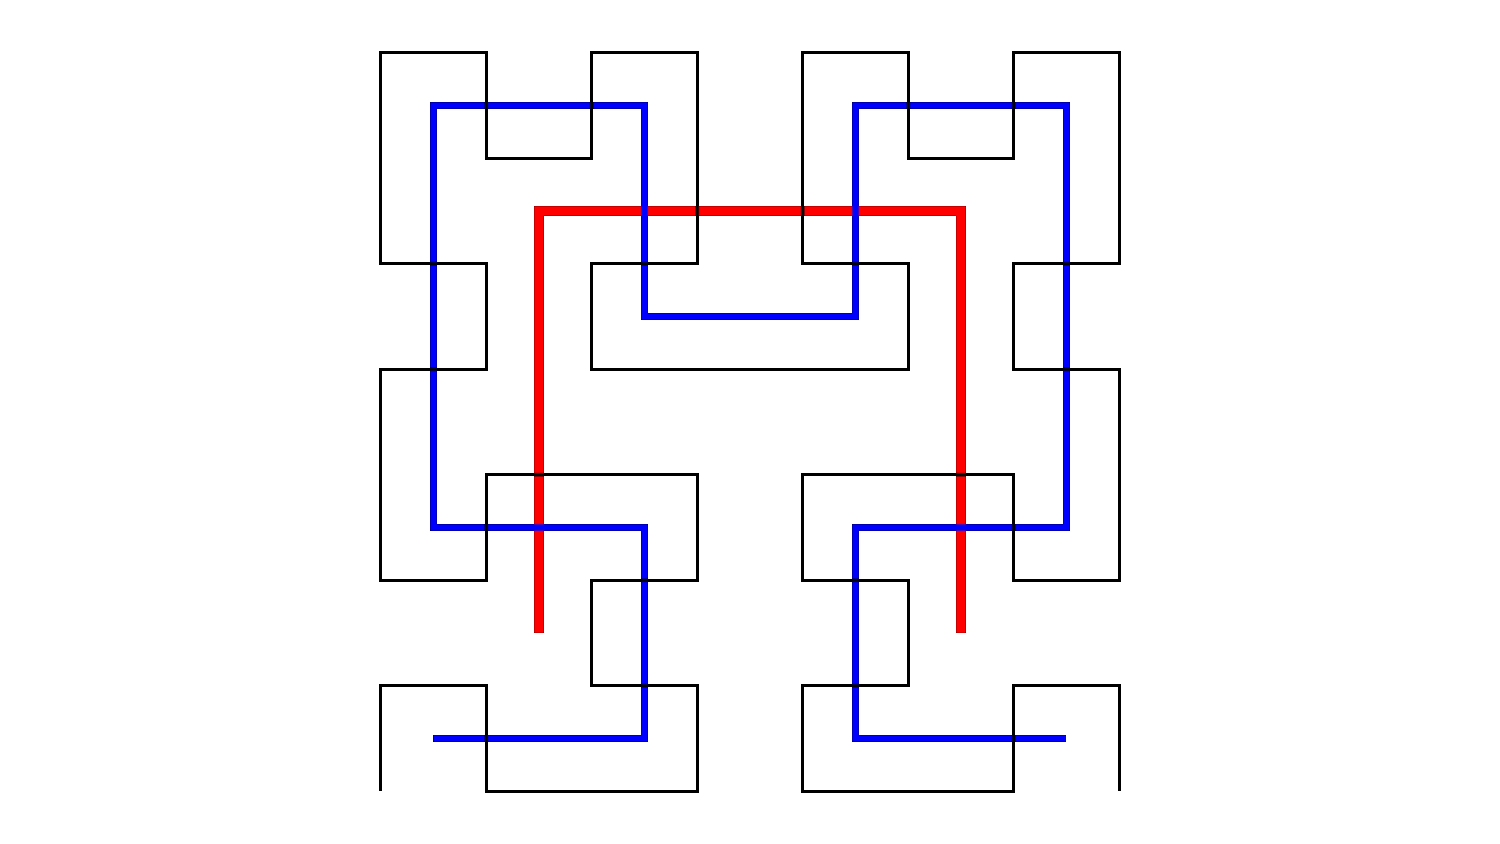
\includegraphics[width=4in]{2d_hilbert.pdf}
\caption{}
\label{fig:2d_hilbert}
\end{figure}